\documentclass[12pt]{article}
\usepackage{amsmath,amssymb,amsthm}
\usepackage{graphicx,mathabx}
\usepackage{xcolor}
\usepackage{tikz}
\usepackage{placeins}
\usepackage{lipsum}
\usepackage[shortlabels]{enumitem}
\begin{document}
\title{TCSS 343 - Week 0}
\author{Jake McKenzie}
\maketitle
\noindent\centerline{\textbf{Recursion with some Asymptotics}}\\\\\\\\\\\\
\begin{center}
    ``So plant your own gardens and decorate your own soul, instead of waiting for someone to bring you flowers." \\$\dots$\\ Jorge Luis Borges
\end{center}
\begin{center}
    ``It's known in theory that $\log{\log{n}}$ approaches infinity, \\but no one has ever observed it in practice." \\$\dots$\\ Grant Sanderson (3blue1brown on youtube)
\end{center}
\begin{center}
Listen to the \textbf{MUSTN'TS}, child,\\
      Listen to the \textbf{DON'TS}\\
      Listen to the \textbf{SHOULDN'TS}\\
The \textbf{IMPOSSIBLES}, the \textbf{WONT'S}\\
      Listen to the \textbf{NEVER HAVES}\\
Then listen close to me-\\
      Anything can happen, child,\\
      \textbf{ANYTHING} can be\\ 
      $\dots$\\
      Shel Silverstein 
\end{center}
    \newpage
\noindent 0. Emily loves figuring out all the ways to arrange dominos. Help her find all the ways to arrange dominos in that are $2 \times 1$ in a $2 \times 1$,$2 \times 2$,$2 \times 3$ and $2 \times 4$ grid!\\\\\\\\\\\\\\\\\\\\\\\\
\noindent 1. Now that you've helped Emily find how many ways to arrange the dominos in problem 0 she gets really philosophical. She starts pondering the nature of zero and wants you to help her find how many ways to arrange a $2 \times 1$ domino in a $2 \times 0$ grid. (You don't have to be too smart: Just find some justification from problem 0)\\\\\\\\\\\\\\\\
\noindent 2. We've had a lot of fun arranging dominos but now Emily wants a recursive formula for the ways to arrange $2 \times 1$ dominos. The key to finding recursive definitions is to find the answer to larger problems by finding the answer to smaller problems.\\\\
$D_n = $\# of tilings of a $2 \times n =$
\newpage
\noindent 3. Show that the left hand side is equal to the right hand side. 
There are two popular tactics in showing such an equality that I've run across. 
The more work but zombie tactic I like is expansion then contraction of both sides then using
the steps you found on the right to be the steps for the left but in reverse. By the fundamental theorem of algebra
both sides must be equal if their full expansions are equal. The other slightly
trickier and requires you to do more thinking up front by trying to find a common factor
in a clever way. Both methods are perfectly valid. Your method may be completely different and valid too.
I'm just trying to give you insight on how to start.
$$\bigg(\frac{k(k + 1)}{2}\bigg)^2\frac{2k^2+2k-1}{3} + (k + 1)^5=\big(\frac{(k+1)(k + 2)}{2}\big)^2\frac{2k^2+5k+2}{3} $$

\newpage
\noindent 4. Calculate the following anti-derivatives from $1$ to $n$ with respect to $x$. (Because I am a nice person. Remember that $\log_2{x}=\frac{\ln{x}}{\ln{2}}$). I have run into all of these integrals when computing runtimes of algorithms, I know you didn't expect this to be so much math but please, please don't hate me. I added these because I care.
\begin{enumerate}
    \item[a)]$6+7x+2x^2$
    \item[b)]$2^n$
    \item[c)]$\log_{2}{x}$
    \item[d)]$\frac{1}{x^2}$
    \item[e)]$\frac{1}{x}$
    \item[f)]$\frac{\log_{2}{x}}{x}$
\end{enumerate}
\newpage
\noindent 5. \textbf{Compute this number: $\log_{2}{\log_{2}{(2^{16})^{(2^{16})!}}}$.} I'll give you some hints:
It is hard to compute exactly by hand but accurate approximations can be found by many different methods, the power $(2^{16})!$ itself has $287,194$ digits where $16,380$ of the tail digits are zero.
What I'm trying to get across with this example is the power of the logarithm vs exponential functions. If you get stuck try to come up
with an approximate answer which is perfectly okay. \textbf{Say you had a $\log{\log{n}}$ algorithm (for example binary search 
which we will look at soon) could you
run this algorithm on this many inputs given a reasonable amount of time?} A single processor core in your computer can perform cca(core cannibalization architecture) $2 \cdot 10^9$ operations per second.
\newpage
\noindent 6. Calculate the second derivative of the product $f(n) \cdot g(n)$ with respect to n. Expand and collect like terms.\\\\\\\\\\\\\\\\\\\\\\\\\\\\\\\\
\noindent 7. Use your result from 7 to calculate the second derivative of the product $f(n) = n + 1$ and $g(n)=e^{2n}$.\\\\\\\\\\\\\\\\\\\\\\\\
\noindent 8. How many operations did you save by using the general result you obtained vs not using it? Do you see why we might want to generalize this result into an algorithm we could apply to classes of problems?
\newpage
\centerline{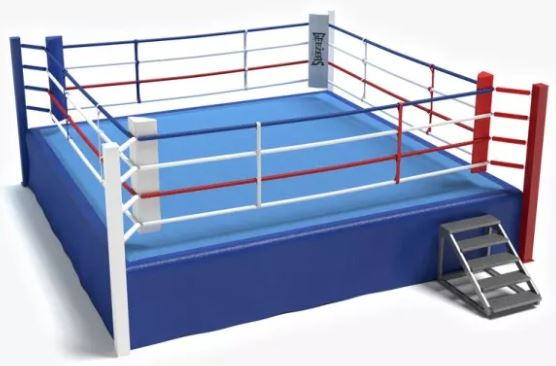
\includegraphics[scale = 0.25]{boxing.jpg}}
\noindent 9. Let's say we have a group of champions in a room and we want to find the best and worst fighter in the room. Now we're betting people and to do this in the quickest way possible. The naive algorithm will use $(n-1) + (n-1) = 2n -2 $ comparisons. We want to do better than that. This is analogous to finding the max value and minimum value in an array of integers. Write a simple recursive algorithm which returns back the max and min, attempt to do it in better than $2n-2$ comparisons.\\\\\\\\\\\\\\\\\\\\\\\\\\
\noindent A. Attempt to prove that this algorithm is correct by contradiction. 
\newpage
\noindent B. Benin is a fisherman who is simply good at fishing. One day, he finds a nice place to go fishing with two ponds. 
Moving from the $i-th$ fish-pond (the one he starts at) to the $j-th$ fishpond would cost $|i - j|$ units of time. 
Initially Benin can get $F_i$ fish in the $i-th$ fishpond. 
In the next turn at the same fishpond, the amount of fish he can get is decreased by $D_i$. 
Notice that Benin will not get negative amount of fish.
Each turn of fishing takes Benin 1 unit of time if Benin is at that pond and $|i - j|$ units of time to switch.
\\\\
For example, if $F_1 = 10$, $F_2 = 5$, $D_1 = 2$, $D_2 = 3$ and Benin can fish for up to eight units of time, then he will get $10 + 8 + 6 + 5 + 4 = 33$.
Washington Department of Fish and Wildlife (WDFW) requires that Benin switch to the adjacent pond when it has more fish and he cannot fish for "negative" fish.
Write a recursive algorithm to see how many fish Benin can fish for!
\newpage
\noindent C. On the last page we had lots of fun but let's get a little more practical. Programmers, no matter what language they use, typically think of their data in trees. Whether their is a collection of JSON objects, Python dicts or Ruby hashes, they're usually a tree. Javascript developers may even take their JSON objects and render them to the DOM, which also happens to be a tree. Trees, trees and more trees. Write a function using recursion that returns true if the tree is symmetric. I encourage you to write as many helper functions as you want.\\
\centerline{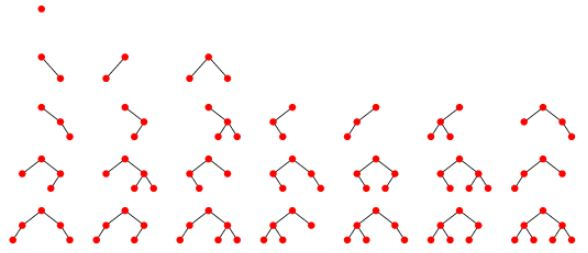
\includegraphics[scale = 0.5]{binarytree.jpg}}
\centerline{(Various binary trees courtesy of Wolfram Mathworld)}
\newpage
\noindent D. Now that you've done this attempt to write a function which will invert a binary tree using recursion.\\
\centerline{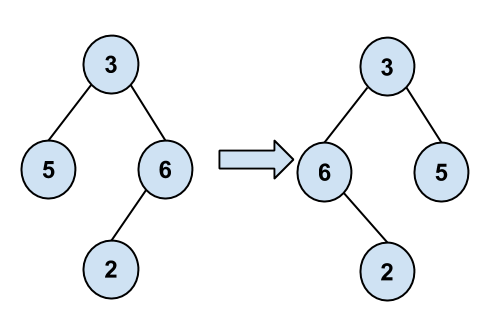
\includegraphics[scale = 0.4]{invertbtree.png}}
\newpage
\noindent E. I'm sorry for making you go through this packet. To be honest I've never been a fan of recursion myself but it is a powerful tool in solving problems. Now that you've completed the previous part of the packet. Reattempt problem 7 by now writing an iterative way of inverting a binary tree.
\centerline{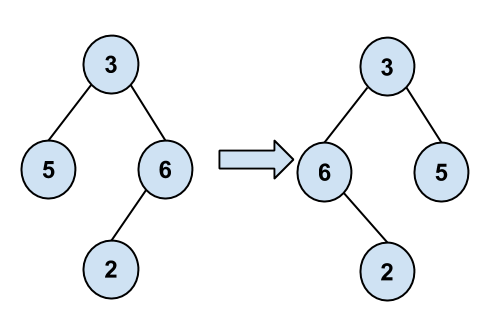
\includegraphics[scale = 0.4]{invertbtree.png}}
\end{document}